\documentclass{article}
\usepackage{hyperref}
\usepackage[utf8]{inputenc}
\usepackage[margin=12.7mm]{geometry}
\usepackage{helvet}
\usepackage{graphicx}
\usepackage{color}
\graphicspath{ {./images/} }
\renewcommand{\familydefault}{\sfdefault}
\author{G12}
\title{Specifica dei requisiti}
\date{}
\begin{document}
\maketitle
\tableofcontents
\clearpage
\section{Scopo del documento}
Il precedente documento riporta la specifica dei requisiti di sistema del progetto Smartfit in linguaggio naturale, in italiano. Per quanto ci si
possa impegnare con costrutti linguistici, la lingua naturale è senza dubbio ambigua quando si tratta di concretizzare delle idee e molte volte dà
grande spazio a interpretazioni personali. Per questo motivo il presente documento ha l'obiettivo di riportare le stesse specifiche, facendo però
uso di diagrammi in Unified Modeling Language (UML) e tabelle strutturate. Per quanto riguarda i requisiti funzionali ci si affiderà a dei
diagrammi UML seguiti da descrizioni accurate, invece per i requisiti non funzionali si farà uso di tabelle strutturate.
\section{Requisiti funzionali}
In questo capitolo si farà uso della lingua italiana e Use Case Diagram (UCD) scritti in UML per riportare i requisiti funzionali.
\begin{itemize}
   \item[RF 1] L'applicazioen Smartfit dovrà essere compatibile con smartphone.
   \item Il sistema dovrà comprendere due tipi di utente:
   \begin{itemize}
      \item Utente base;
      \item Allenatore;
   \end{itemize}
   \item[RF 2] Registrazione al sistema.
   \item[RF 3] Accesso al sistema.
   \item[RF 4] Recupero dati di accesso.   
   \item[RF 12] Registrazione allenatore. 
   \begin{center}
      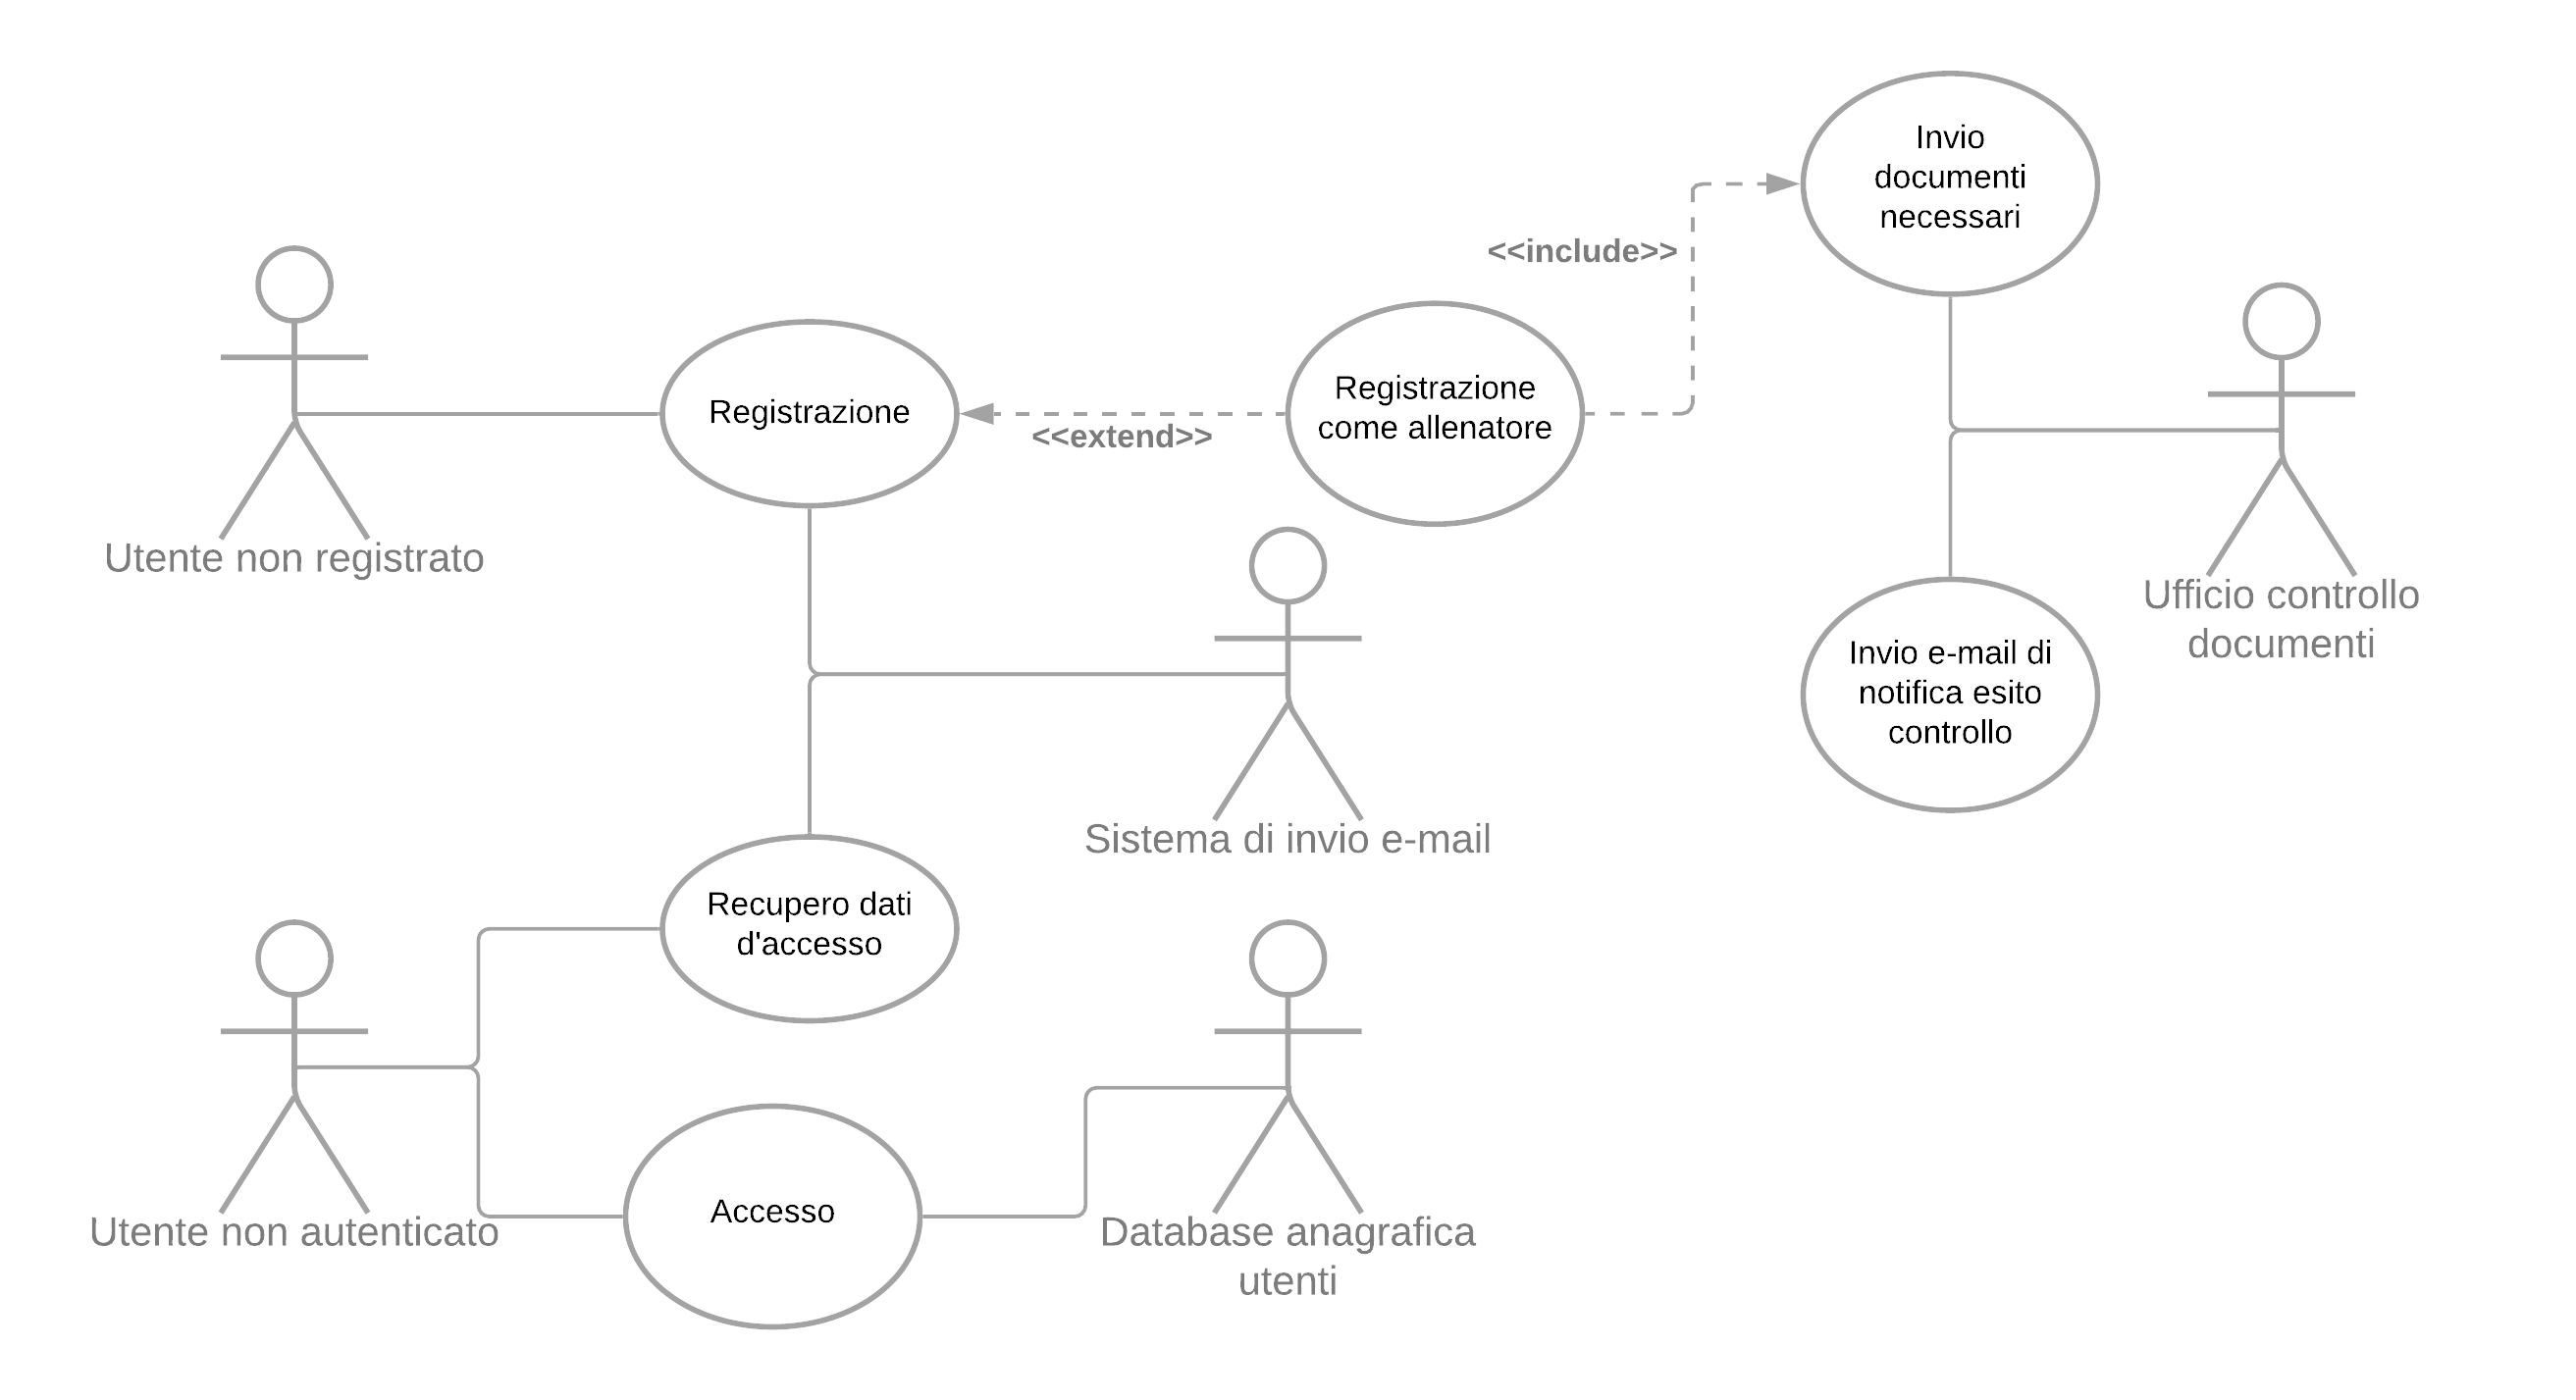
\includegraphics[width=175mm]{Utente non registrato.png}
   \end{center}
\end{itemize}
\textbf{Descrizione Use Case "Registrazione"}\\
\\
Titolo: Registrazione\\
\\
Riassunto:\\
Questo use case descrive come avviene la registrazione di un nuovo utente.\\
\\
Descrizione: \\
Al primo accesso al sistema verrà presentata una schermata di registrazione dove sarà possibile creare un account inserendo username [exception 3],
email e password (le ultime due da ripetere due volte) [exception 1] [exception 2], oltre ai dati come nome, cognome, data di nascita, peso,
altezza, sesso, unità di misura (kg/m o lb/ft) necessari per il funzionamento dell’applicazione. Dopo aver completato questo passaggio, con l’ausilio
di un sistema esterno, verrà inviata una mail all’indirizzo specificato con un link per completare la registrazione; una volta cliccato, il processo
sarà completato [exception 4]. I dati di accesso verranno salvati in un database esterno.\\
\\
Exceptions:\\
$[$exception 1$]$Se l’indirizzo email inserito dall’utente è già associato a un account esistente, l’utente deve essere notificato di ciò e
invitato a procedere con il login.\\
$[$exception 2$]$ Se le due email o le due password non coincidono, l’utente viene notificato e invitato a reinserirle per poter proseguire.\\
$[$exception 3$]$ Se lo username è già associato a un account, l’utente viene notificato e può scegliere di accedere (nel caso in cui fosse il suo)
oppure cambiarlo con uno nuovo.\\
$[$exception 4$]$ Se non viene aperto il link inviato via email per la conferma della registrazione, l’utente non può continuare e l’account non
viene creato.\\
\newline
\newline
\textbf{Descrizione Use Case "Invio documenti necessari"}\\
\newline
Titolo: Invio documenti necessari.\\
\newline
Riassunto:\\
Questo use case descrive come avviene la registrazione come allenatore.\\
\\
Descrizione: \\
All’atto dell’iscrizione, se si è un allenatore, si potrà spuntare una checkbox in cui si autocertificherà come tale. Con questa opzione attivata
si aprirà una sezione aggiuntiva nel form in cui sarà necessario caricare i documenti che provano la propria professione. Questi documenti verranno
poi inviati automaticamente all’ufficio predisposto per la validazione, che procederà al controllo ed eventualmente alla conferma. L’allenatore
potrà comunque utilizzare l’applicazione come utente base mentre attende il riconoscimento.\\
\\
Extensions:\\
$[$extension 1$]$ L’esito del controllo dei documenti da parte dell’ufficio predisposto verrà inviato all’utente sia come notifica push sia
via e-mail (inviata direttamente dall’ufficio). Se i documenti vengono approvati, le nuove funzionalità (quelle da allenatore) verranno rese
accessibili nell’applicazione automaticamente.\\
\\
\\
\textbf{Descrizione Use Case "Accesso"}\\
\\
Titolo: Accesso\\
\\
Riassunto:\\
Questo use case descrive come l’utente deve accedere avendo già un account\\
\\
Descrizione:\\
Al primo accesso se si sceglie di accedere con account già esistente o negli accessi successivi al primo sarà presentata una schermata dove sarà
possibile l’accesso all’applicazione mediante username (o email) e password.\\
\\
Extensions:\\
$[$extension1$]$ Sarà presente una checkbox per memorizzare le credenziali e non doverle ripetere agli accessi successivi.\\
\\
\\
\textbf{Descrizione Use Case "Recupero dati d’accesso"}\\
\\
Titolo: Recupero dati d’accesso\\
\\
Riassunto:\\
Questo use case descrive come viene eseguito il recupero dei dati d’accesso\\
\\
Descrizione:\\
Nel caso si siano dimenticati i dati d’accesso (username e/o password), nella schermata d’accesso sarà presente un link per resettarli ed inserirne
di nuovi, utilizzando l’email scelta al momento della registrazione. Nella mail che verrà inviata automaticamente ci sarà un link che aprirà una
schermata in-app per il ripristino dei dati d’accesso.
\\
\\
\begin{itemize}
   \item[RF 5] Visualizzazione riepilogo kilocalorie.
   \item[RF 6] Visualizzazione cronologia kilocalorie assunte/bruciate.
   \item[RF 7] Aggiunta e rimozione pasto e attività fisica.
   \item[RF 8] Rilevamento automatico attività fisica.
   \item[RF 9] Visualizzazione scheda personalizzata.
   \item[RF 10] Visualizzazione allenatore.
   \item[RF 11] Modifica profilo utente.
   \item[RF 13] Generazione ed eliminazione scheda.
   \item[RF 14] Invio scheda.
   \item[RF 15] Aggiunta e rimozione allievo.
   \item[RF 16] Visualizzazione andamento utente.
   \begin{center}
      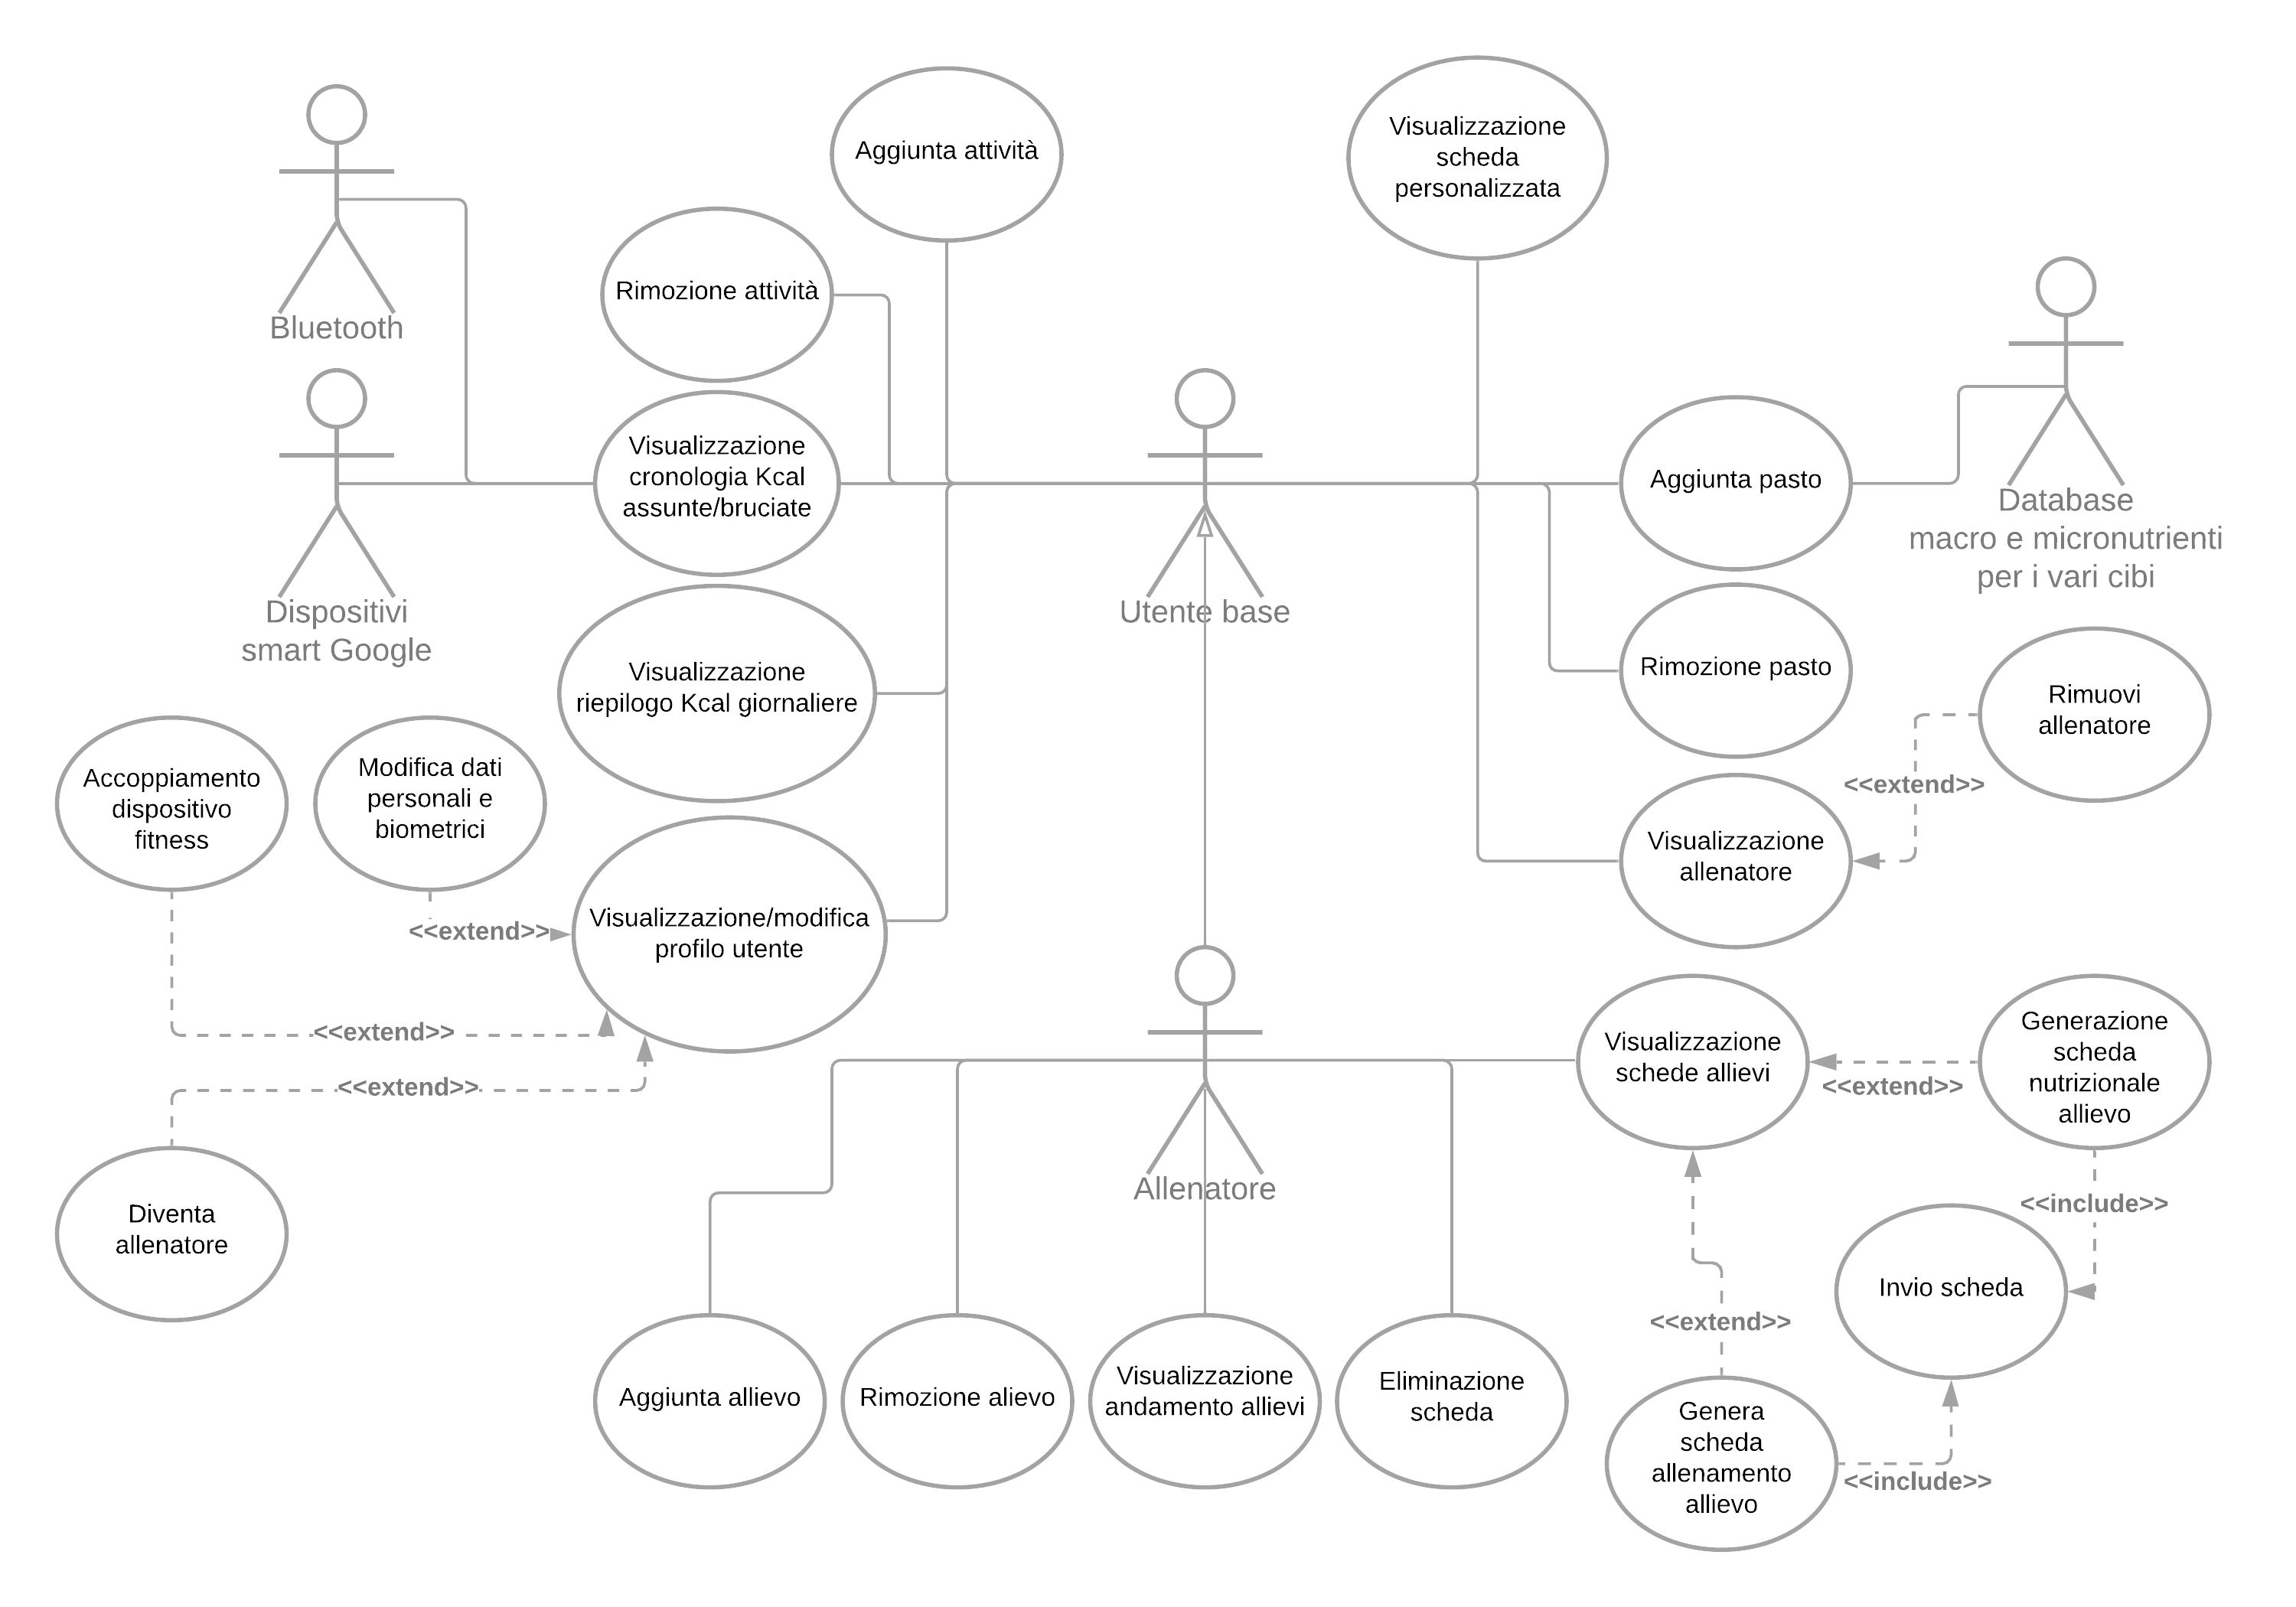
\includegraphics[width=175mm]{Utente base.png}
   \end{center}
\end{itemize}
\textbf{Descrizione Use Case "Aggiunta attività"}\\
\newline
Titolo: \\
Aggiunta attività\\
\\
Descrizione:\\
Per l’aggiunta di un’attività fisica sarà richiesta la tipologia (ad esempio “passeggiata” o “corsa”) e il numero di kcal bruciate.\\
\\
\\
\textbf{Descrizione Use Case "Aggiunta pasto"}\\
\\
Titolo:\\
Aggiunta pasto\\
\\
Descrizione: \\
Per l’aggiunta di un pasto verrà richiesto il nome del piatto e la quantità consumata (espressa in grammi, centilitri,.. a seconda della tipologia
di cibo) e il sistema provvederà a calcolare la percentuale di macro e micronutrienti assunti ed inserirli nella cronologia e nel grafico iniziale.
Per questo calcolo l’applicazione si baserà sull’utilizzo di un database, come indicato successivamente; in questo database ogni pietanza è
associata ai corrispondenti valori nutrizionali\\
\\
\\
\textbf{Descrizione Use Case "Visualizzazione allenatore"}\\
\\
Titolo:\\
Visualizzazione allenatore\\
\\
Descrizione:\\ 
L’utente potrà visualizzare i dettagli del proprio allenatore (nome, età, …)\\
\\
\\
\textbf{Descrizione Use Case "Rimuovi allenatore"}\\
\\
Titolo:\\
Rimuovi allenatore\\
\\
Descrizione:\\ 
L’utente potrà rimuovere l’allenatore ed eventualmente sostituirlo con un altro. Ad ogni utente potrà essere associato un solo allenatore per volta.
Si ricordi inoltre che non è l’utente che aggiunge l’allenatore bensì il contrario. L’allenatore invia una richiesta all’allievo e se questo lo
accetta allora diventa il suo allenatore.\\
\\
\\
\textbf{Descrizione Use Case "Visualizzazione cronologia Kcal assunte/bruciat"}\\
\\
Titolo:\\
Visualizzazione cronologia Kcal assunte/bruciate\\
\\
Riassunto:\\
Questo use case descrive come l’utente può visualizzare la propria cronologia di Kcal assunte e bruciate\\
\\
Descrizione:\\
L’utente potrà vedere un elenco che consiste nella cronologia dell’attività fisica intrapresa (kcal bruciate) e dei pasti consumati (kcal assunte).
Ogni voce descriverà la tipologia di attività (per esempio passeggiata o pranzo) e il numero di kcal rispettivamente assunte o perse a seconda
dell’attività. Sarà inoltre possibile visualizzare la cronologia dei giorni precedenti senza la possibilità di aggiungere o eliminare voci. I dati
dopo 14 giorni vengono eliminati automaticamente, quindi la cronologia parte dalla voce più recente filo a quella risalente a 14 giorni prima. Le
attività fisiche svolte mediante l’utilizzo di dispositivi fitness accoppiato tramite Bluetooth verranno automaticamente categorizzate ed inserite
nella cronologia, con le relative Kcal bruciate. Per la comunicazione Bluetooth con i dispositivi smart vengono utilizzate le API di Google Fit.\\
\\
\\
\textbf{Descrizione Use Case "Visualizzazione riepilogo Kcal giornaliere"}\\
\\
Titolo:\\
Visualizzazione riepilogo Kcal giornaliere\\
\\
Riassunto:\\
Questo use case descrive come l’utente può visualizzare il riepilogo Kcal giornaliere\\
\\
Descrizione:\\
In un grafico l’utente potrà visualizzare la percentuale di kilocalorie assunte durante la giornata, suddivise per tipologia di macronutrienti
(proteine, carboidrati e grassi). Cliccando su un pulsante verrà reso disponibile anche l’elenco dei micronutrienti assunti (per esempio vitamine,
ferro,...).\\
\\
\\
\textbf{Descrizione Use Case "Visualizzazione scheda personalizzata"}\\
\\
Titolo:\\
Visualizzazione scheda personalizzata\\
\\
Riassunto:\\
Questo use case descrive come l’utente può visualizzare la propria scheda personalizzata\\
\\
Descrizione:\\
L’utente potrà visualizzare una o più schede ricevute dal proprio allenatore. Le schede includono una dieta personalizzata in base a macro e
micronutrienti ed indicazioni sul movimento o sugli esercizi per quanto riguarda l’attività fisica. Si ricordi che un allievo può avere solo una
scheda per tipologia alla volta, ovvero una di alimentazione e una di allenamento.\\
\\
\\
\textbf{Descrizione Use Case "Visualizzazione/modifica profilo utente"}\\
\\
Titolo:\\
Visualizzazione/modifica profilo utente\\
\\
Riassunto:\\
Questo Use Case descrive cosa può fare l’utente in termini di modifica del suo profilo e anche delle impostazioni generali dell’applicazione\\
\\
Descrizione:\\ 
L’utente può visualizzare le informazioni associate al suo profilo ed eventualmente cambiarle.
\begin{enumerate}
    \item L’utente può cambiare i suoi dati personali come email e password e i dati biometrici. Per questioni di spazio è stato omesso l’attore
            del database eterno di anagrafica, ad ogni modo il database deve essere aggiornato con le nuove modifiche apportate.
    \item L’utente può inviare una richiesta per diventare allenatore come spiegato nello Use Case “Diventa allenatore”.
    \item L’utente può cambiare le unità di misura utilizzate nell’applicazione (kg/m e lb/ft).  Dopo aver modificato la preferenza sulle unità di
            misura verrà effettuata in automatico la conversione dei dati già inseriti.
\end{enumerate}
\bigskip
\textbf{Descrizione Use Case "Diventa allenatore"}\\
\\
Titolo:\\
Diventa allenatore\\
\\
Descrizione:\\
Questo Use Case è analogo a quello “Registrazione come allenatore” visto nello UCD di registrazione. Per questioni di spazio è stato omesso tutto il
contorno che riguarda questo use case, si prenda come riferimento lo UCD sopracitato nel quale è stato descritto tutto nel dettaglio di come i
documenti vengono inviati all’ufficio di verifica e come quest’ultimo invia la notifica dell’esito.\\
\\
\\
\textbf{Descrizione Use Case "Accoppiamento dispositivo fitness"}\\
\\
Titolo:\\
Accoppiamento dispositivo fitness\\
\\
Descrizione:\\
L’utente avrà la possibilità di accoppiare dispositivi fitness per il rilevamento automatico dell’attività fisica tramite Bluetooth.\\
\\
\\
\textbf{Descrizione Use Case "Aggiunta allievo"}\\
\\
\\
Titolo:\\
Aggiunta allievo\\
\\
Riassunto:\\ 
Questo use case descrive come un allenatore aggiunge un allievo\\
\\
Descrizione:\\
Un allenatore può ricercare per username o email gli utenti ed inviare una richiesta per associarsi a loro. Gli utenti riceveranno una notifica
push e in-app e una volta accettata quell’allenatore sarà associato a quell’utente e potrà inviargli le schede e visualizzare il suo andamento
giornaliero. Un allenatore può avere associati più utenti base.\\
\\
\\
\textbf{Descrizione Use Case "Visualizzazione andamento allievi"}\\
\\
Titolo:\\
Visualizzazione andamento allievi\\
\\
Riassunto:\\
Questo use case descrive come un allenatore visualizza l’andamento dei propri allievi\\
\\
Descrizione:\\
L’allenatore avrà accesso rapido agli utenti a cui è associato, e schiacciando su ognuno di loro gli verrà presentata la stessa schermata
principale degli utenti base, in modo che possa monitorare l’andamento dell’utente. Ovviamente non avrà a disposizione i pulsanti per aggiungere o
rimuovere i pasti e l’attività fisica.\\
\\
\\
\textbf{Descrizione Use Case "Generazione scheda allievo"}\\
\\
Titolo:\\
Generazione scheda allievo\\
\\
Riassunto:\\
Questo use case descrive come un allenatore crea una scheda personalizzata per un suo allievo\\
\\
Descrizione:\\
Ad un allenatore dovrà essere permessa la generazione di una scheda nutrizionale e/o di allenamento personalizzata, in cui indicherà il numero di
kcal da assumere giornalmente e anche dei piatti consigliati per assumere il corretto quantitativo di macro e micronutrienti. Sarà inoltre possibile
aggiungere anche un piano di attività fisica personalizzato sulla base dell’utente a cui sarà indirizzato.\\
\\
\\
\textbf{Descrizione Use Case "Invio scheda"}\\
\\
Titolo:\\
Invio scheda\\
\\
Descrizione:\\
Questo use case vale sia per le schede di allenamento che per quelle nutrizionali, l’unica cosa che cambia è il documento inviato. Una volta creata
una scheda personalizzata da parte di un allenatore, questa deve essere inviata a uno o più utenti base che riceveranno una notifica push e in-app
di avvenuta consegna.\\
\\
\\
\textbf{Descrizione Use Case "Eliminazione scheda"}\\
\\
Titolo:\\ 
Eliminazione scheda\\
\\
Descrizione:\\ 
Una volta creata una scheda, essa rimarrà associata e visualizzabile da parte dell’allenatore nella schermata di creazione scheda dove si può
eliminare.\\
\section{Requisiti non funzioanli}
\begin{itemize}
    \item [RNF 1] \textbf{Sicurezza}\\
                 \begin{tabular}{|p{5cm}|p{8cm}|p{5cm}|}
                     \hline
                     Proprietà & Descrizione & Misura\\
                     \hline
                     Blocco account & Se l’utente sbaglia la password per un certo numero di volte, l’account va bloccato per un certo periodo.&
                     Dopo 3 errori consecutivi, l’account viene bloccato per 24 ore\\
                     \hline
                     Recupero password & Se l’utente dimentica la password d’accesso, deve essere possibile cambiarla & Sistema recupero password descritto precedentemente\\
                     \hline
                     Protezione credenziali & Le password vengono crittografate quando salvate nel database & Utilizzo protocollo https per le comunicazioni con il database anagrafico degli utenti\\
                     \hline
                     Password sicura&La password deve essere una strong password&La password deve rispettare determinati requisiti. Deve essere lunga almeno 10 caratteri e contenere almeno un numero e un carattere speciale\\
                     \hline
                 \end{tabular}
   \item [RNF 2] \textbf{Privacy}\\
                 \begin{tabular}{|p{5cm}|p{11cm}|p{2cm}|}
                     \hline
                     Proprietà & Descrizione & Misura\\
                     \hline
                     Codice della privacy & Il codice per la protezione dei dati personali(informalmente noto anche come "codice della privacy"), 
                     di cui al Decreto legislativo 30 giugno 2003, n. 196 , in vigore dal 1º gennaio 2004, contiene le norme nazionali relative alla
                     tutela dei dati personali. & Conforme\\
                     \hline
                     Regolamento per la protezione dei dati (GDPR) & Il Garante per la protezione dei dati personali ha elaborato una versione
                     "arricchita" del testo del Regolamento (UE) 2016/679, che - laddove necessario - segnala in corrispondenza di articoli e
                     paragrafi i relativi "Considerando" di riferimento, in modo da offrire una lettura più ampia e ragionata delle previsioni
                     introdotte dalla nuova normativa. Aggiornato alle rettifiche pubblicate sulla Gazzetta Ufficiale dell'Unione europea 127 del
                     23 maggio 2018. & Conforme\\
                     \hline
                     Accesso limitato & I dati dell’utente possono essere visualizzati solamente dall’utente stesso e dal proprio allenatore &
                     Conforme\\
                     \hline
                     Comunicazioni client-server sicure & Vengono criptate per prevenire l’eventuale intercettazione di dati sensibil & 
                     Utilizzo protocollo https per ogni connessione effettuata\\
                     \hline
                 \end{tabular}
   \item [RNF 3] \textbf{Scalabilità}\\
                 \begin{tabular}{|p{5cm}|p{11cm}|p{2cm}|}
                     \hline
                     Proprietà & Descrizione & Misura\\
                     \hline
                     Elaborazione con un numero crescente di utenti & L’applicazione deve essere in grado di adattarsi ad un numero crescente di
                     utenti, per garantire la qualità e la velocità del servizio & parte da 100,000 utenti a 1,000,000\\
                     \hline
                 \end{tabular}
   \item [RNF 4] \textbf{Operatività}\\
                 \begin{tabular}{|p{5cm}|p{11cm}|p{2cm}|}
                     \hline
                     Proprietà & Descrizione & Misura\\
                     \hline
                     Tempo di funzionamento & Si intende il tempo massimo in cui il sistema è raggiungibile & 24 ore su 24\\
                     \hline
                     Tempo massimo verifica documenti allenatore & Tempo massimo di risposta all’utente che ha deciso di registrarsi come allenatore & 
                     Massimo 1-2 giorni lavorativi\\
                     \hline
                 \end{tabular}
   \item [RNF 5] \textbf{Memorizzazione dati}\\
                 \begin{tabular}{|p{5cm}|p{11cm}|p{2cm}|}
                     \hline
                     Proprietà & Descrizione & Misura\\
                     \hline
                     Database esterno&l’applicazione salva i dati degli utenti (credenziali registrazione, schede, cronologia delle kcal assunte/bruciate) in un database esterno, per garantire il recupero dei dati in caso di disinstallazione e successiva reinstallazione dell’applicazione&Conforme\\
                     \hline
                 \end{tabular}
   \item [RNF 6] \textbf{Multilingua}\\
                 \begin{tabular}{|p{5cm}|p{8cm}|p{5cm}|}
                     \hline
                     Proprietà & Descrizione & Misura\\
                     \hline
                     Multilingua & La lingua dell’applicazione verrà rilevata automaticamente dal dispositivo & Se la lingua di sistema è l’italiano allora le schermate saranno in italiano altrimenti in inglese\\
                     \hline
                 \end{tabular}
   \item [RNF 7] \textbf{Prestazioni}\\
                 \begin{tabular}{|p{5cm}|p{10cm}|p{3cm}|}
                     \hline
                     Proprietà & Descrizione & Misura\\
                     \hline
                     Avvio applicazione & Tempo massimo di avvio dell’applicazione sul proprio smartphone & Una volta avviata l’applicazione, deve essere disponibile in
                     massimo 2 secondi\\
                     \hline
                     Cambio schermata & Tempo massimo quando l’utente decide di cambiare la schermata attuale, magari visualizzando la propria scheda &
                     Massimo 1.5 secondi\\
                     \hline
                     Tempo massimo login & Tempo massimo adibito alla schermata di login, dopo il quale viene visualizzato un messaggio d’errore &
                     Massimo 7 secondi, dopodiché si ritorna automaticamente alla schermata di login\\
                     \hline
                 \end{tabular}
   \item [RNF 8] \textbf{Compatibilità}\\
                 \begin{tabular}{|p{5cm}|p{11cm}|p{2cm}|}
                     \hline
                     Proprietà & Descrizione & Misura\\
                     \hline
                     Compatibilità con Android & Sistema operativo e versione dalla quale l’applicazione risulta disponibile sullo store ufficiale &
                     A partire da Android 5.0\\
                     \hline
                 \end{tabular}
   \item [RNF 9] \textbf{Affidabilità}\\
                 \begin{tabular}{|p{5cm}|p{10cm}|p{3cm}|}
                    \hline
                     Proprietà & Descrizione & Misura\\
                    \hline
                    Ritentare l’operazione&In caso di errore durante il login, la registrazione oppure con l’invio di una scheda, deve essere possibile ritentare l’operazione&Conforme\\
                    \hline
                 \end{tabular}
\end{itemize}
\section{Note}
Questa sezione ha lo scopo di riassumere le modifiche che sono state apportate ai requisiti del progetto (funzionali e non) rispetto al documento
precedente. Preme precisare che le modifiche sono state suggerite da noi, per la maggior parte, soltantoe poi accordate con il gruppo G11 a noi associato e sono univocamente
state apportate perché certi punti non erano sufficientemente chiari o mancavano dei dettagli necessari alla descrizione senza ambiguità degli
stessi.
Per quanto riguarda i requisiti funzionali:
\begin{enumerate}
    \item E' stato precisato che la e-mail di notifica dell'esito del controllo dei documenti di un allenatore da parte dell'ufficio predisposto è
            inviata dallo stesso, non dal sistema. Il sistema quindi si occuperà solo di inviare una notifica in-app.
    \item E' stato chiarito il fatto che per "visualizzare una o più schede ricevute dal proprio allenatore" nel RF9 dello scorso documento si parla
             delle due schede distinte di allenamento e alimentazione, quindi al massimo una scheda per ogni tipologia. Non si possono quindi avere più
            schede di alimentazione o di allenamento.
    \item Abbiamo chiarito che nel RF10 dello scorso documento il metodo di sostituzione di un allenatore è solo di eliminare l'allenatore già
            associato e poi accettare una richiesta di associazione da un altro allenatore. Si può avere al massimo un allenatore alla volta e un utente
            non può cercare un allenatore ma solo il contrario.
    \item E' stato specificato che, per quanto riguarda il RF14 dello scorso documento, l'invio di una scheda è necessario non appena è stata creata.
            Non si può quindi creare una scheda senza poi inviarla.
\end{enumerate}
Per quanto riguarda i requisiti non funzionali c’è stato solo un cambiamento importante:\\
Nel requisito funzionale della sicurezza (RNF1), il gruppo G11 non aveva le idee ben chiare su come dovesse essere gestito il blocco dell’account
dopo i 3 tentativi di accesso falliti perciò si è optato per un blocco temporaneo (24 ore) che comunque funge da sistema di sicurezza contro
attacchi brute force o dizionario.\\
Non sono stati effettivamente modificati altri requisiti non funzionali ma sono state aggiunte delle misure. Nello scorso documento di molti
requisiti non funzionali mancava una quantificazione degli stessi, è stato quindi chiesto al gruppo G11 di fornire delle misure e/o delle stime
per rendere la tabella strutturata sufficientemente dettagliata.\\
\end{document}